\documentclass{article}
\usepackage[utf8]{inputenc}


\title{TACOS}
\author{Julien ALAIMO, Hugo FEYDEL, Olivier HUREAU }
\date{2019-2020}
\usepackage{graphicx}

\begin{document}

\maketitle

\section{Fonctionnalités intéressante/importante}

Le système implémenté est incomplet mais permissif. Certaines erreurs de code ou appel système résulte en une bonne exécution. Cela permet à un programmeur non confirmé de pouvoir tout de même utiliser le système. 

Nous avons aussi implémenté des fonctions systèmes pour les utilisateurs confirmé. Ceux-ci peuvent alors utiliser des structures d'une manière moins intuitive, aux risques et périls de l'utilisateur.



\subsection{Le Multithreading}

Le multiThreading permet à un utilisateur de faire tourner plusieurs instructions en parallèle. Similaire au processus dans un environement linux, les threads partagent le même espace mémoire.

Notre réalisation permet une utilisation simpliste et permissive du multithreading : si certaines mécaniques de fermeture sont oublié, le système le fera par lui même. 

\newpage
\section{Spécifications}

\textit{
une partie "spécifications" listant ce qui est disponible pour les programmes utilisateurs. Il faut mettre ici le genre d'information que vous trouvez dans les pages man. On doit donc trouver tous les appels systèmes implémentés avec leur prototype, la description des arguments, la description du fonctionnement (fonctionnalités utilisateurs, pas implémentation) de l'appel système, de la valeur de retour éventuelle, la signalisation des erreurs, ... Si vous avez également une bibliothèque utilisateur, vous devez décrire ses fonctions de la même manière que les appels systèmes.
}



\subsection{Entrées/Sorties}
\begin{itemize}
    \item 
    \textbf{void PutChar( char c);}
    
    Ecris le charactère "char c" sur la sortie standard
    
    \item 
    \textbf{void PutString(char * string);}
    
    Ecris le chaine de caractère "char * string" sur la sortie standard.
    La chaine de caractère doit finir par '\textbackslash0'.
    La taille maximal de la chaine de caractère est de 
    \textbf{ MODIFIE ICI STP}.
    L'apel système \textbf{PutString} est moins coûteux que plusieurs appels système \textbf{PutChar}
    
     \item 
    \textbf{int GetChar();}
    
    Retourne la valeur ascii d'un caractère rentré dans l'entrée standard.
    La fonction attend qu'un charactère soit disponnible. Attention il peux y avoir blocage.
    
    
     \item 
    \textbf{void GetString(char * string, int taille);}
    
    Ecris la chaine de caractère rentrée dans l'entrée standart à l'adresse de la chaine de caractère en paramètre \textbf{char * string}. La taille de cette chaîne de caractère sera inférieur ou égal au paramètre \textbf{int taille}.
    \textbf{JULIEN MODIFIE ICI, c'est peut etre faux}.
    
      \item 
    \textbf{void GetInt(int * n);}
    
    Ecris l'entier rentrée dans l'entrée standart à l'adresse pointé par le paramètre \textbf{n}.
    L'entier peux être positif comme négatif.
    La valeur absolue de lentier ne dois pas êre supérieur a \[10^{10}-1\] (valeur absolue). Sinon une erreur est levée.
    
    
    
      \item 
    \textbf{void PutInt(int n);}
    
     Ecris l'entier en paramètre \textbf{int n} sur la sortie standard
    L'entier peux être positif comme négatif.
    La valeur absolue de l'entier ne dois pas êre supérieur a \[10^{10}-1\] (valeur absolue). Sinon une erreur est levée.
    
    
\end{itemize}

\subsection{Threads}
Le programmation multithreadé permet à l'utilisateur d'éxecuter plusieurs threads simultanément. Les threads partagent la mémoire virtuelle et l'utilisation du coeur. Chaque thread possède néanmoins son propre fil d'exécution, ses propres registres (dont le pointeur d'instrcution PC) et sa pile.


Tout les threads sont identifié par des identifiants unique stocké sur des unsigned int. A la mort de chaque thread, lors de la mort de son parent, l'identifiant du thread enfant est retransmis au système de gestion des identifiants afin qu'il soit recyclé. Le thread principal ayant pour identifiant '1', si la mémoire le permet, il est possible d'utiliser jusqu'à \(2^{32}-1\) thread simultanément mais aussi possible d'avoir une infinité de thread ayant était éxecuté sur la machine d'un point de vue temporel.

Dans le système tacOS il existe un lien de parenté entre tout les threads. Chaque thread créé est enfant du thread créateur. A la fin de l'exécution d'un thread dis \textit{\textbf{parent}} , celui-ci va attendre la fin de l'exécution de tout ses fils. 

Cependant, un mode \textit{\textbf{survivant}} est mis en place tel que lorsqu'un un thread est dis \textit{\textbf{survivant}}, il ne seras pas attendu pas son thread père met par son grand père. 

Voici les différentes procédures liéé aux threads :
\begin{itemize}
 
    \item 
    \textbf{unsigned int CreateThread(void * f (void * arg), void * arg;}
    
    Crée un thread utilisateur et lance la routine \textbf{f}. Le deuxième argument 
    \textbf{void * arg} est passé en argument a la fonction f.
    Retourne l'identifiant du thread.
   
   \item 
   \textbf{void ExitThread(void * obj)} 
   
   Termine le thread courant et injecte l'adresse de l'objet dans les structures l'adresse \textbf{void * obj} afin qu'un thread parent puisse l'utiliser. Doit être appelé lorsque l'on désire terminer un thread "fils". \textit{Le système possède néanmoins un mécanisme permettant de rattraper cet oubli }
   
   \item 
   \textbf{unsigned int ThreadId();}
   
  Retourne l'identifiant du thread courant.   
   
   \item
   \textbf{void * WaitForChildExited(int CID);} 
   
   Attente passif que le thread d'identifiant \textbf{CID} termine. Retourne une adresse correspondant à l'objet donné par le thread enfant lors de son exit. Si cette adresse est équivalente à \textbf{(void *) -1}, alors l'identifiant \textbf{CID} n'as pas était reconnu où le thread n'est pas enfant.
   
    
\end{itemize}


\begin{itemize}
  \item 
  \textbf{void WaitForAllChildExited();}
  
  Met le thread en attente actif. Le thread sort de l'attente quand plus aucun de ses threads enfants sont en cours d'execution (y compris les thread en mode survivant)
  
  \item 
  \textbf{int StopChild(int CID)}
  
  Met en pause le thread enfant d'identifiant \textbf{CID}. 
  La fonction retourne :    
    \begin{itemize}
      \item \textbf{0} Si succès
      \item \textbf{1} Si l'arrêt à échoué
      \item \textbf{2} Si l'identifiant n'est pas celui d'un de ses enfants
    \end{itemize} 
    Si le thread est en zone critique (Ecriture /lecture) dans la conssole, le thread s'arretera après cette lecture/ecriture.      
    
  
  \item 
  \textbf{int WakeUpChild(int CID);}
  
    
  Reveil le thread enfant d'identifiant \textbf{CID}. 
  La fonction retourne :    
    \begin{itemize}
      \item \textbf{0} Si succès
      \item \textbf{1} Si l'identifiant n'est pas celui d'un de ses enfants
      \item \textbf{2} Si le thread n'est pas en pause
    \end{itemize} 
    
  
  \item 
  \textbf{int makeChildSurvive(int CID);}
  
  Met le thread enfant d'identifiant \textbf{CID} en \textbf{mode survivor} jusqu'à la mort du père .
  
  \item 
  \textbf{void makeAllChildSurvive();}
  
  Met tout les threads enfant en \textbf{mode survivor} jusqu'à la mort du père courant.
\end{itemize}

\subsection{Système de fichiers}

\newpage
\section{Tests Utilisateurs}
\textit{une partie "tests utilisateurs" décrivant les programmes de test que vous avez réalisés, ce qu'ils montrent, ...}
\vspace{5mm}

\subsection{Threads}

\begin{itemize}
	\item Le test de la class \textit{\textbf{ List} (que nous avons modifié)} se lance avec l'argument -tl. Ce test va vérifier si : Un liste retourne le bon boolean lors de l'appel de IsEmpty(), les éléments ont bien était ajouté dans le bon ordre, les éléments ont bien était supprimé dans le bon ordre, la fonction ajouté get(index) fonctionne correctement. \textit{voir testImplem.cc}


\item Le test de la class \textbf{UserThreadManagerId} se lance avec l'argument -utmmono. Ce test va vérifier si : Le manager commence au bon endroit, les identifiants sont recyclés, un identifiant recyclé est donné en priorité par rapport à un nouvel indentifiant. \textit{voir testImplem.cc}

\item \textbf{CreateAndReturn.c} : Ce test vérifie qu'un Thread se crée correctement et que sa valeur de retour est juste.
	
\item \textbf{ExitWithoutStatement.c} : Ce test vérifie que même lorsqu'un thread n'utilise pas d'appel de retour (return ou ExitThread), celui-ci se termine correctement.
	
\item \textbf{MultiGetChar.c} : Ce test vérifie la spécification de la console and mode multithreadé : Plusieurs getString sont lancé en même temps, on vérifie que l'execution de celle-ci est bien de manière séquentiel.

	
\item \textbf{Survive.c} : Ce test vérifie que l'implémentation du mode survivor fonctionne correctement. Le fils doit écrire sur le terminal avec que le petit fils ait finis d'écrire.
	
\item \textbf{WaitForThread.c} : Ce test vérifie que les parents attendent bien que leurs fils se terminent (un seul père, 2 fils)

\item \textbf{WaitForThreadMulti.c} : Ce test vérifie que les parents attendent bien que leurs fils se terminent (un seul père, 1 fils, 1 petit fils)
		
		\item \textbf{Sleep.c} : Ce test vérifie qu'un thread père peux bien mettre en attente un fils : Le fils est programmé pour ecrire en continu sur la console, le StopThread() arrète donc bien l'enfant de parler.

\item \textbf{Wake.c} :	Ce test vérifie père peux bien réveiller son fils.
		
	
	

\end{itemize} 

\newpage
\section{Implémentation}
\textit{une partie "implémentation" qui explique les points importants de votre implémentation. C'est donc la seule partie qui parle du détail du code que vous avez écrit. Expliquez vos choix d'implémentation.
}
\vspace{5mm}

\subsection{Threads}




Pour implémenter les threads, nous avons choisis d'utiliser les 3 classes suivantes
\begin{itemize}
\item
UserThread
\item
ManagerUserThreadID
\item
UserThreadData
\end{itemize}
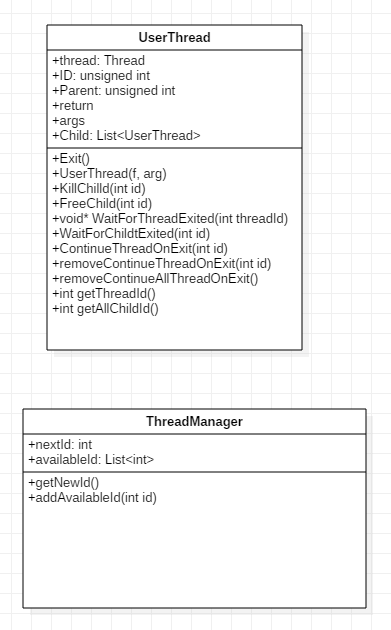
\includegraphics{code/userprog/UserThread.PNG}

Ainsi, chaque thread utilisateur sera associé à un thread kerbel grâce au stockage de l'adresse d'un UserThread dans la classe Thread du Kernel


Lorsqu'un appel système se déclenche, via le pointeur machine->currentThread ou se trouve un pointeur vers son UserThread, on pas alors utiliser les UserThread pour y appliquer les différentes opérations nécessaire.
\vspace{5mm}

L'assignation des identifiants d'UserThread se fait via le UserThreadManager. Le userThreadManager stock un variable compteur qui est incrémenter à chaque demande d'identifiant. C'est UserThread étant stocké sur des "unsigned int" on peux se voir limiter en nombre de thread parallèle par la limite de taille d'un unsigned int. Cependant, les identifiants sont recyclé. A chaque destruction de UserThread on réinjecter alors sont identifiant dans la liste du ThreadManager. Cela permet alors d'être sur qu'on programme à longue utilisation ne se retrouve jamais à cours d'identifiant. Néanmoins cela implique une plus grosse structure de stockage et une éventuelle perte temps par rapport à d'autre structure (exemple : bitmap)

\section{Scolaire}
\textit{une partie plus "scolaire" où vous décrivez l'organisation de votre travail (planning, ...), commentaires constructifs sur le déroulement du projet, ...}
\vspace{5mm}

\end{document}
